\chapter{Flow Control}
During this chapter implementation and evaluation of various control algorithms for flow control purposes will be presented. At first, the aim is to enable regulation of flow to a constant value. Later on, the system's ability to follow different reference flow trajectories will be tested. In a final step, the system will be subjected to disturbancees through the HiL test rig in form of heart beats at different heart rates. Performances of the implemented control algorithms will be compared.

\section{Controller Design}
As a first step towards flow control implementation two versions of PI controllers are implemented to ensure stable system behavior. After comparing the performance results of both approaches, a parallel approach to ILC implementation, under use of the higher performing PI controller, is applied to improve the follow up behavior and reduce control errors.

\subsection{PI Controller}
PI control implementation is performed on the basis of the tuning rules according to Ziegler Nichols (see chapter \ref{chap:ZN}), as well as according to Chien Hrones Reswick (Chapter \ref{chap:CHR}).
\\As a preparation for the utilization of the inflection tangent methods for these tuning approaches a measurement similar to the one for determination of the static map is performed. \figurename~\ref{fig:dyn_meas} depicts the signal curves for the determination of the tuning parameters. As presented in the upper graph differential pressure is increased in steps of $20\,mmHg$ from $\Delta{p}=0\,mmHg$ to $\Delta{p}=100mmHg$. For each level the sequence of reference velocities depicted examplary for $\Delta{p}=40\,mmHg$ in the center graph of \figurename~\ref{fig:dyn_meas_40} is targeted. Starting at $v_{ref}=4000 \, rpm $ the velocity is in three steps of varying height first increased and  then decreased by the same value. The first step amounts to $200 \, rpm$, the second to $400\,rpm$ and the third to $600 \, rpm$. The reference value is then increased by $1000\,rpm$ and again the three steps are executed. This sequential behavior is repeated up to a start value of $v_{ref}=800\,rpm$.

\begin{figure}[ht]
  \centering
  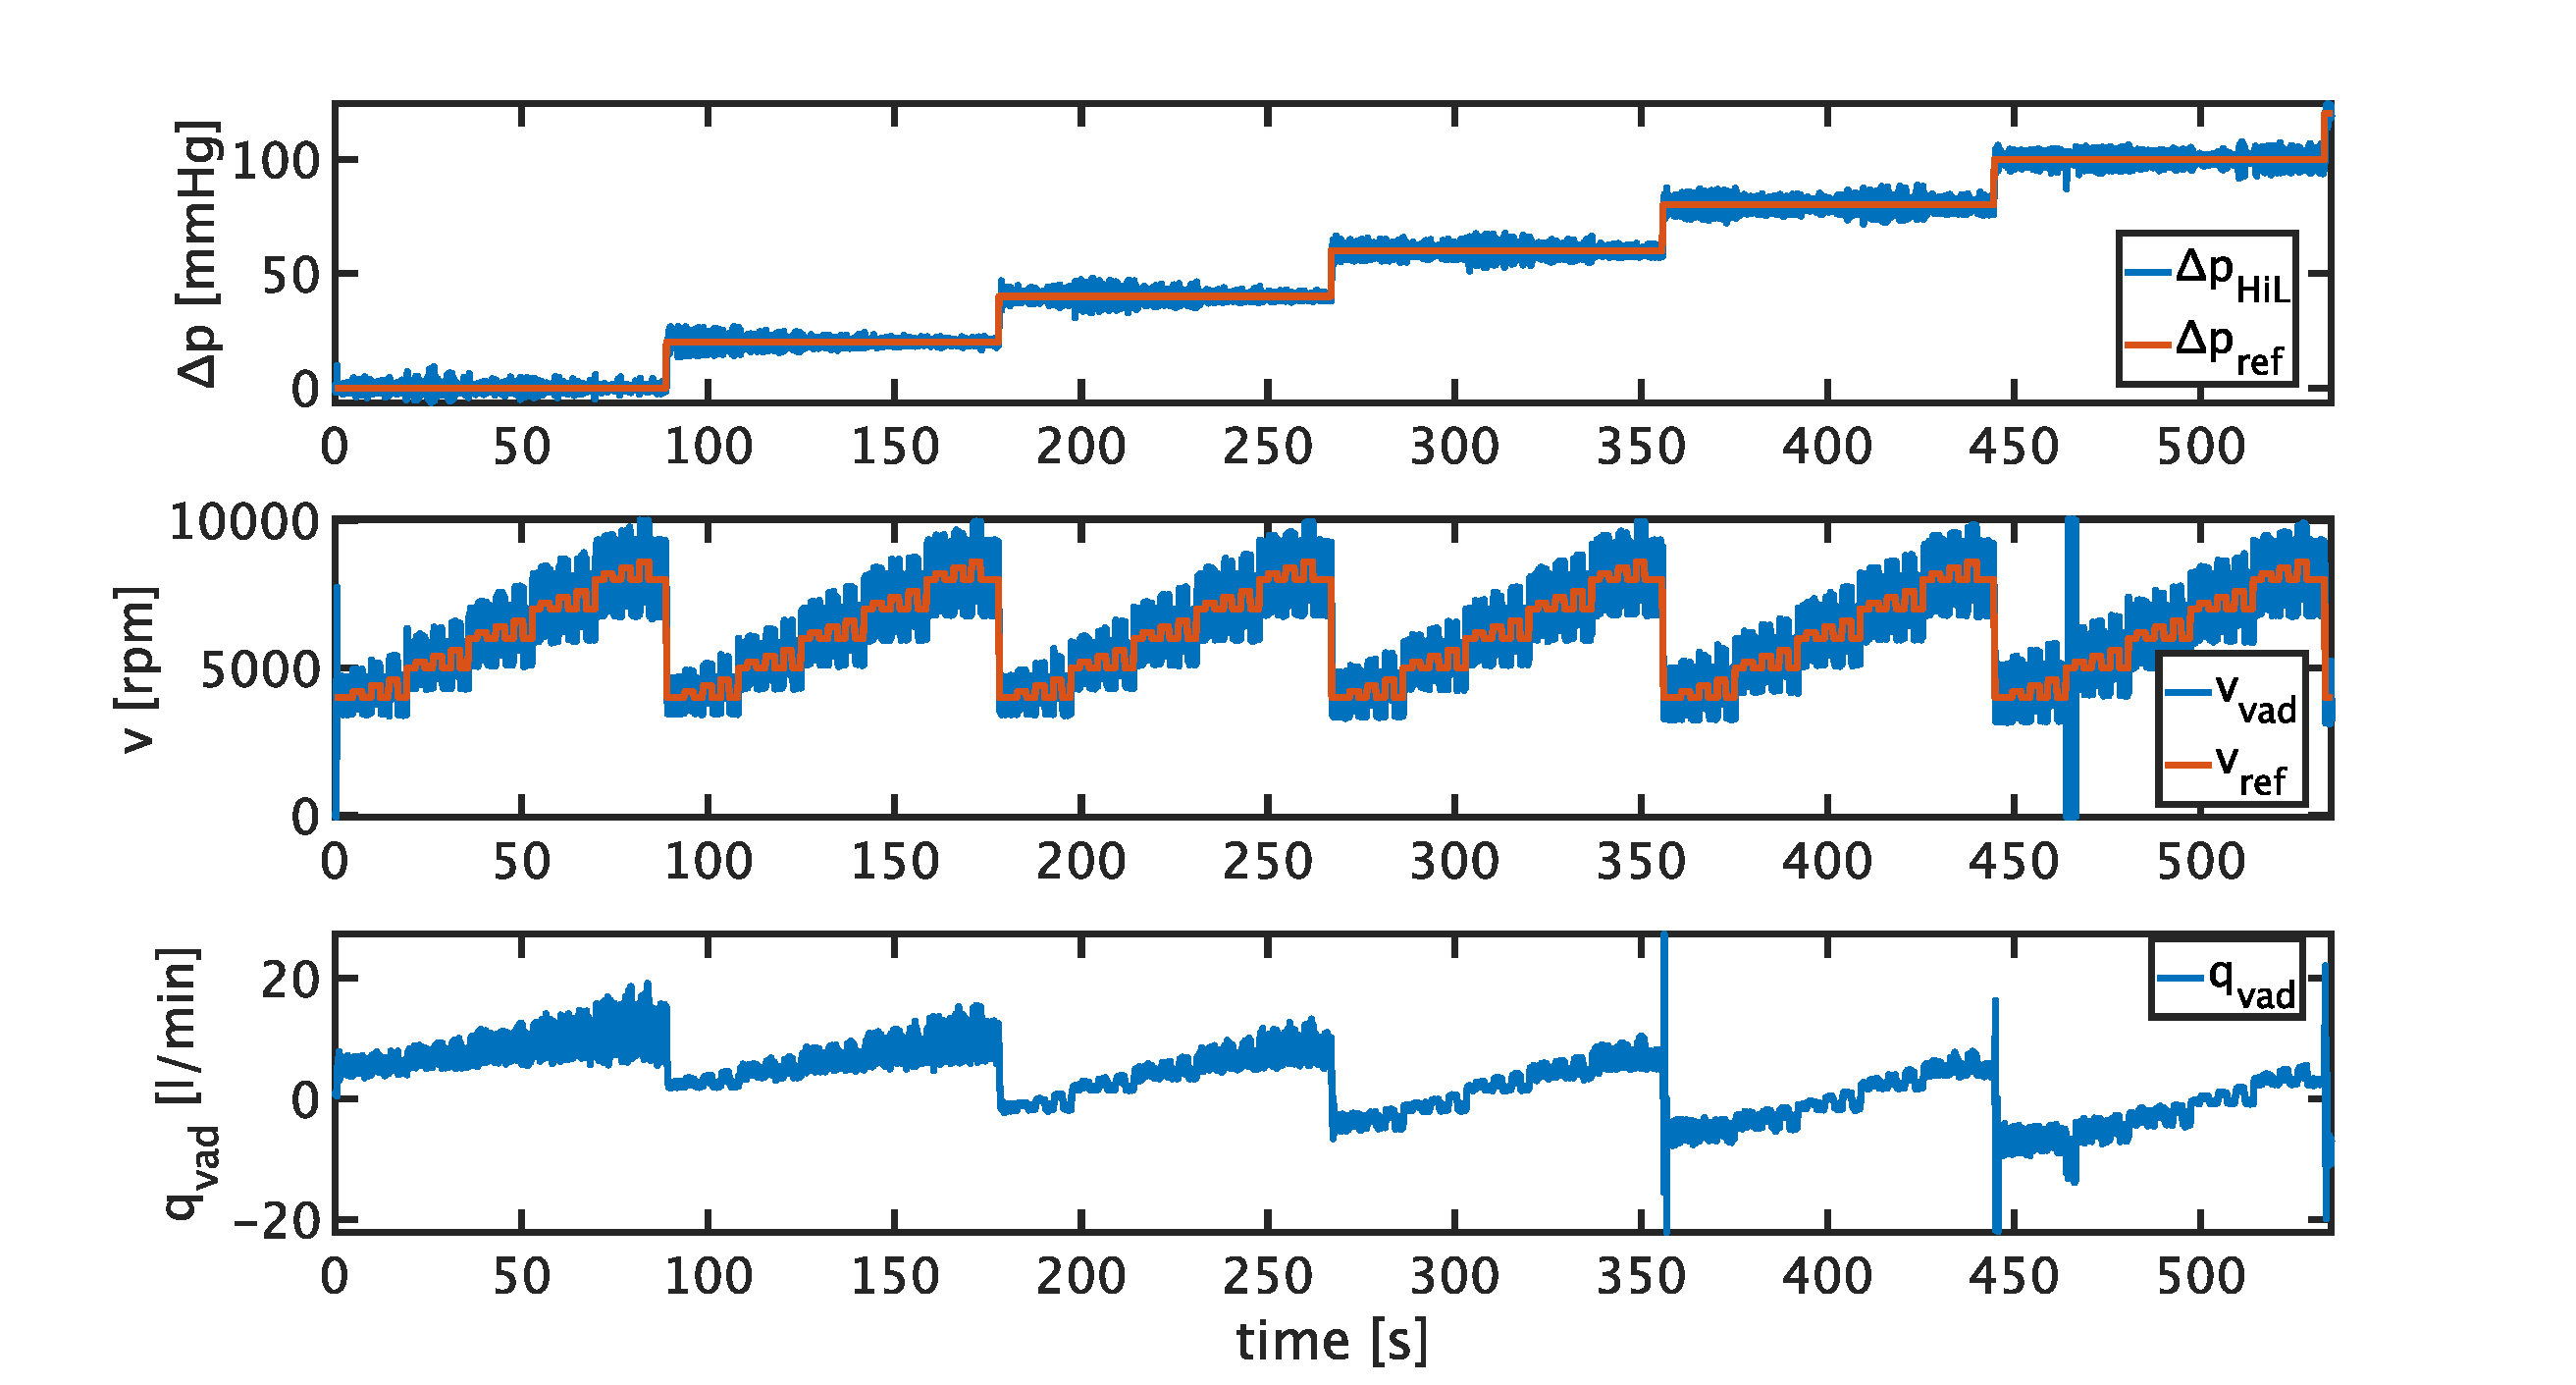
\includegraphics[width=\textwidth]{images/chapt_5/dyn_measure.pdf}
  \caption[Signal curves for determination of PI controller parameters]{Signal curves for determination of PI controller parameters. Top: differential pressure as reference and measured signal, middle: reference and measured rotational speed, bottom: measured flow through Sputnik VAD.}
  \label{fig:dyn_meas}
\end{figure}

\begin{figure}[ht]
  \centering
  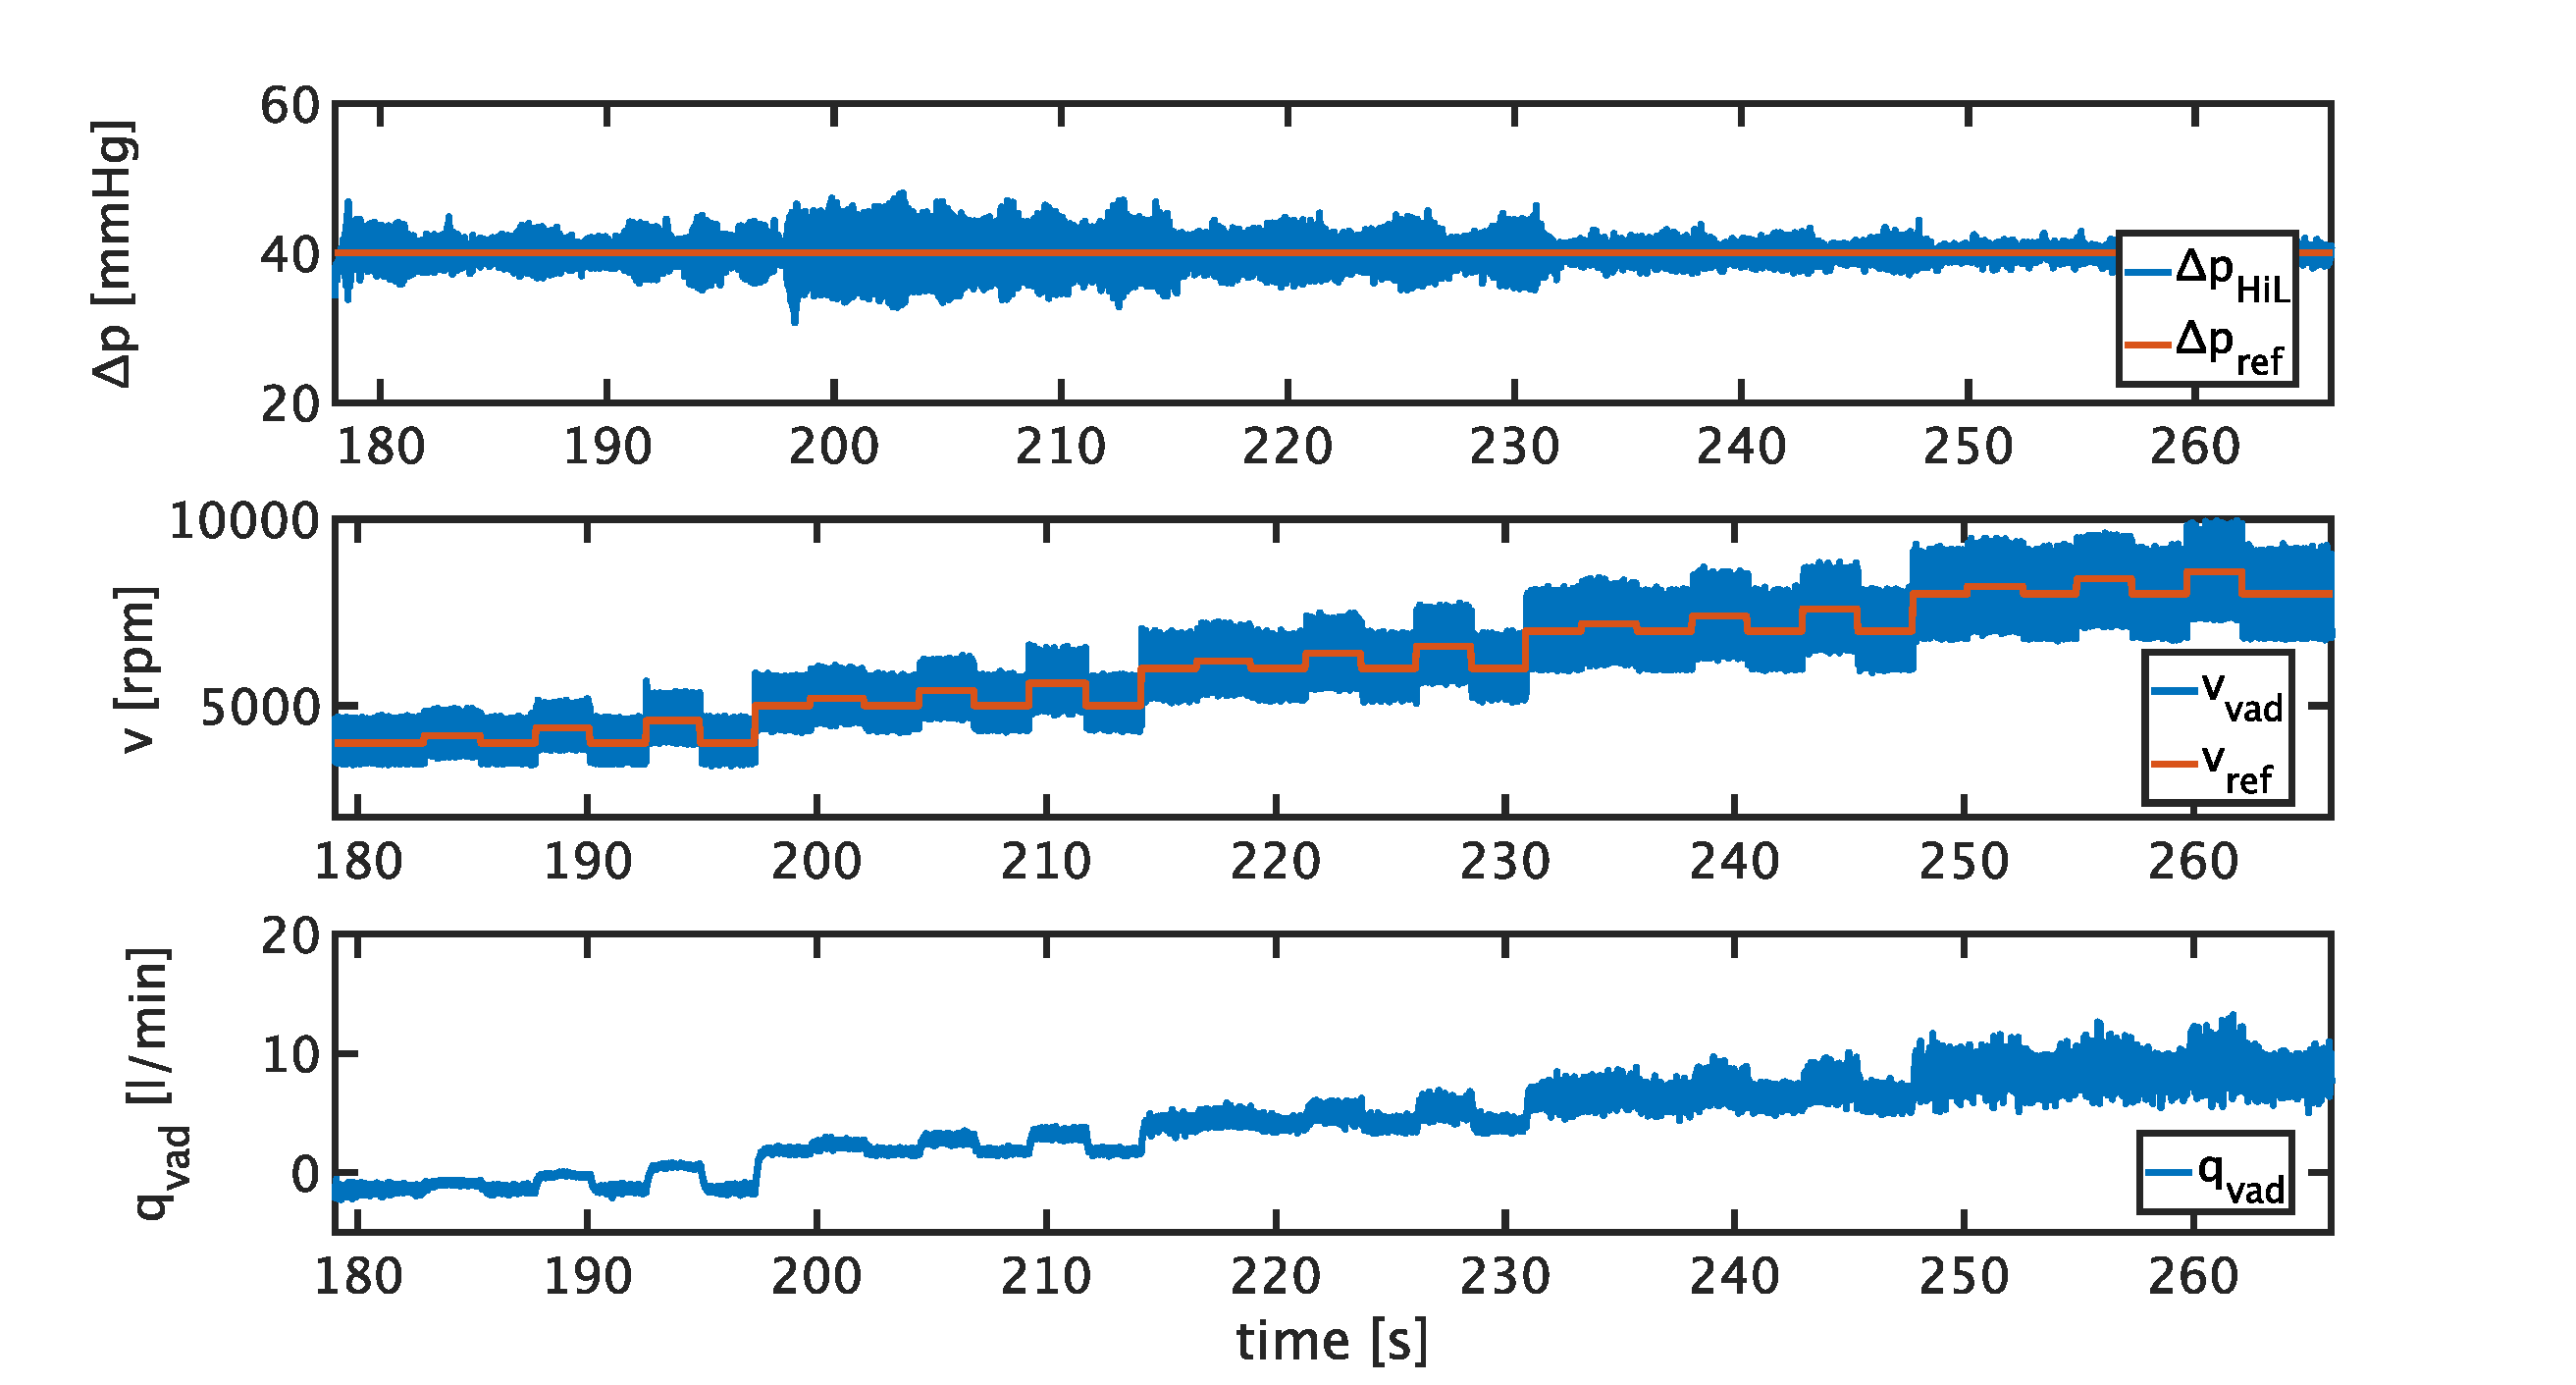
\includegraphics[width=\textwidth]{images/chapt_5/dyn_meas_40.pdf}
  \caption[Signal curves for determination of PI controller parameters at $\Delta{p}=40\,mmHg$]{Signal curves for determination of PI controller parameters at $\Delta{p}=40\,mmHg$.}
  \label{fig:dyn_meas_40}
\end{figure}

For the determination of the parameters for the controller design the step from $v_{ref,low}=5000\, rpm$ to $v_{ref,high}=5400\, rpm$ at $\delta{p}=40mmHg$, which is located in the center of the pump's opeating range, is used.
Since the measured flow signal has a high measurement noise, the sigal is preprossed using an $8^{th}$-order butterworth filter with cut off frequency $f_c=5Hz$ and sampling frequency $f_s=1000Hz$. The resulting signal and the characteristic parameters needed for parameter tuning of the PI controller are depicted in \figurename~\ref{fig:param_calc_PI}.

\begin{figure}[ht]
  \centering
  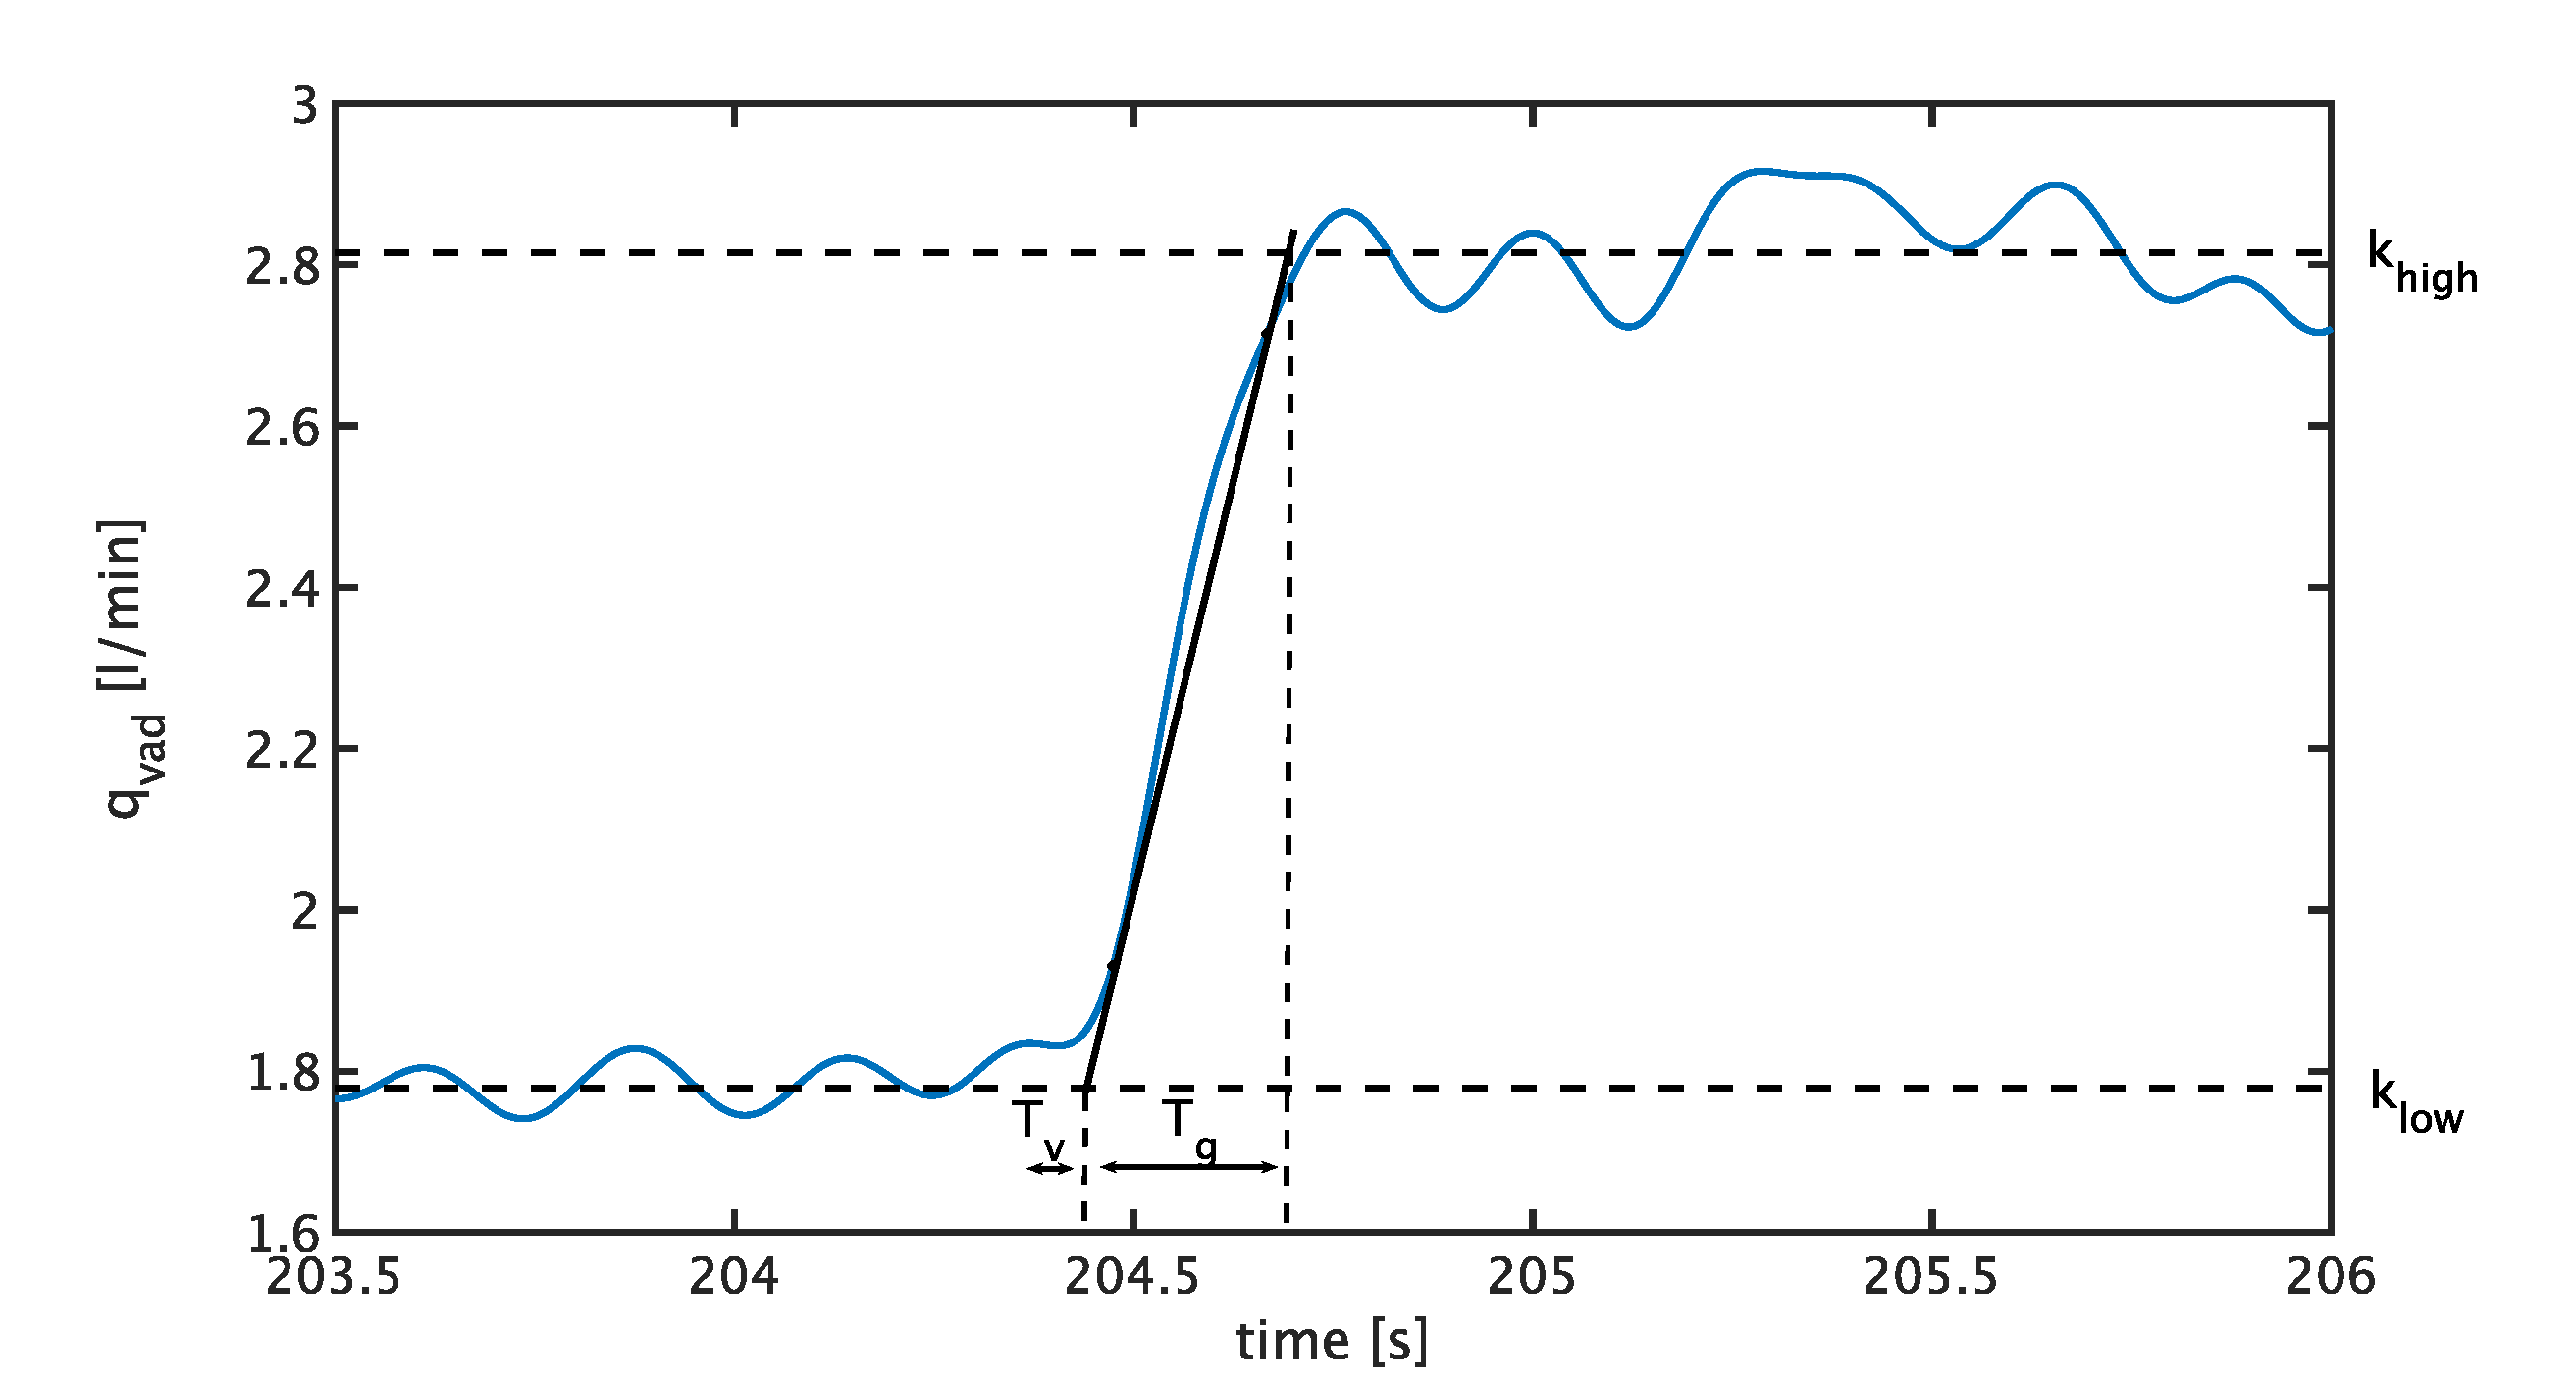
\includegraphics[width=\textwidth]{images/chapt_5/param_calc_PI.pdf}
  \caption[Step response for determination of PI controller tuning parameters]{Step response for a step in rotational speed of $400\,rpm$ for determination of PI controller tuning parameters.}
  \label{fig:param_calc_PI}
\end{figure}

% Dynamische Messung nutzen
% Werte an Sprungstellen
% Nach Wendetangenten verfahren -> GRAFIK
%Berechnung erklären
\subsection{Iterative Learning Control}

\subsection{Iterative Learning Control with varying iteration length}

\section{Evaluation}
\subsection{PI Controller}
gesamt:
rms pi total chr = 0.3705
rms pi total zn = 0.5396
\begin{figure}[ht]
  \centering
  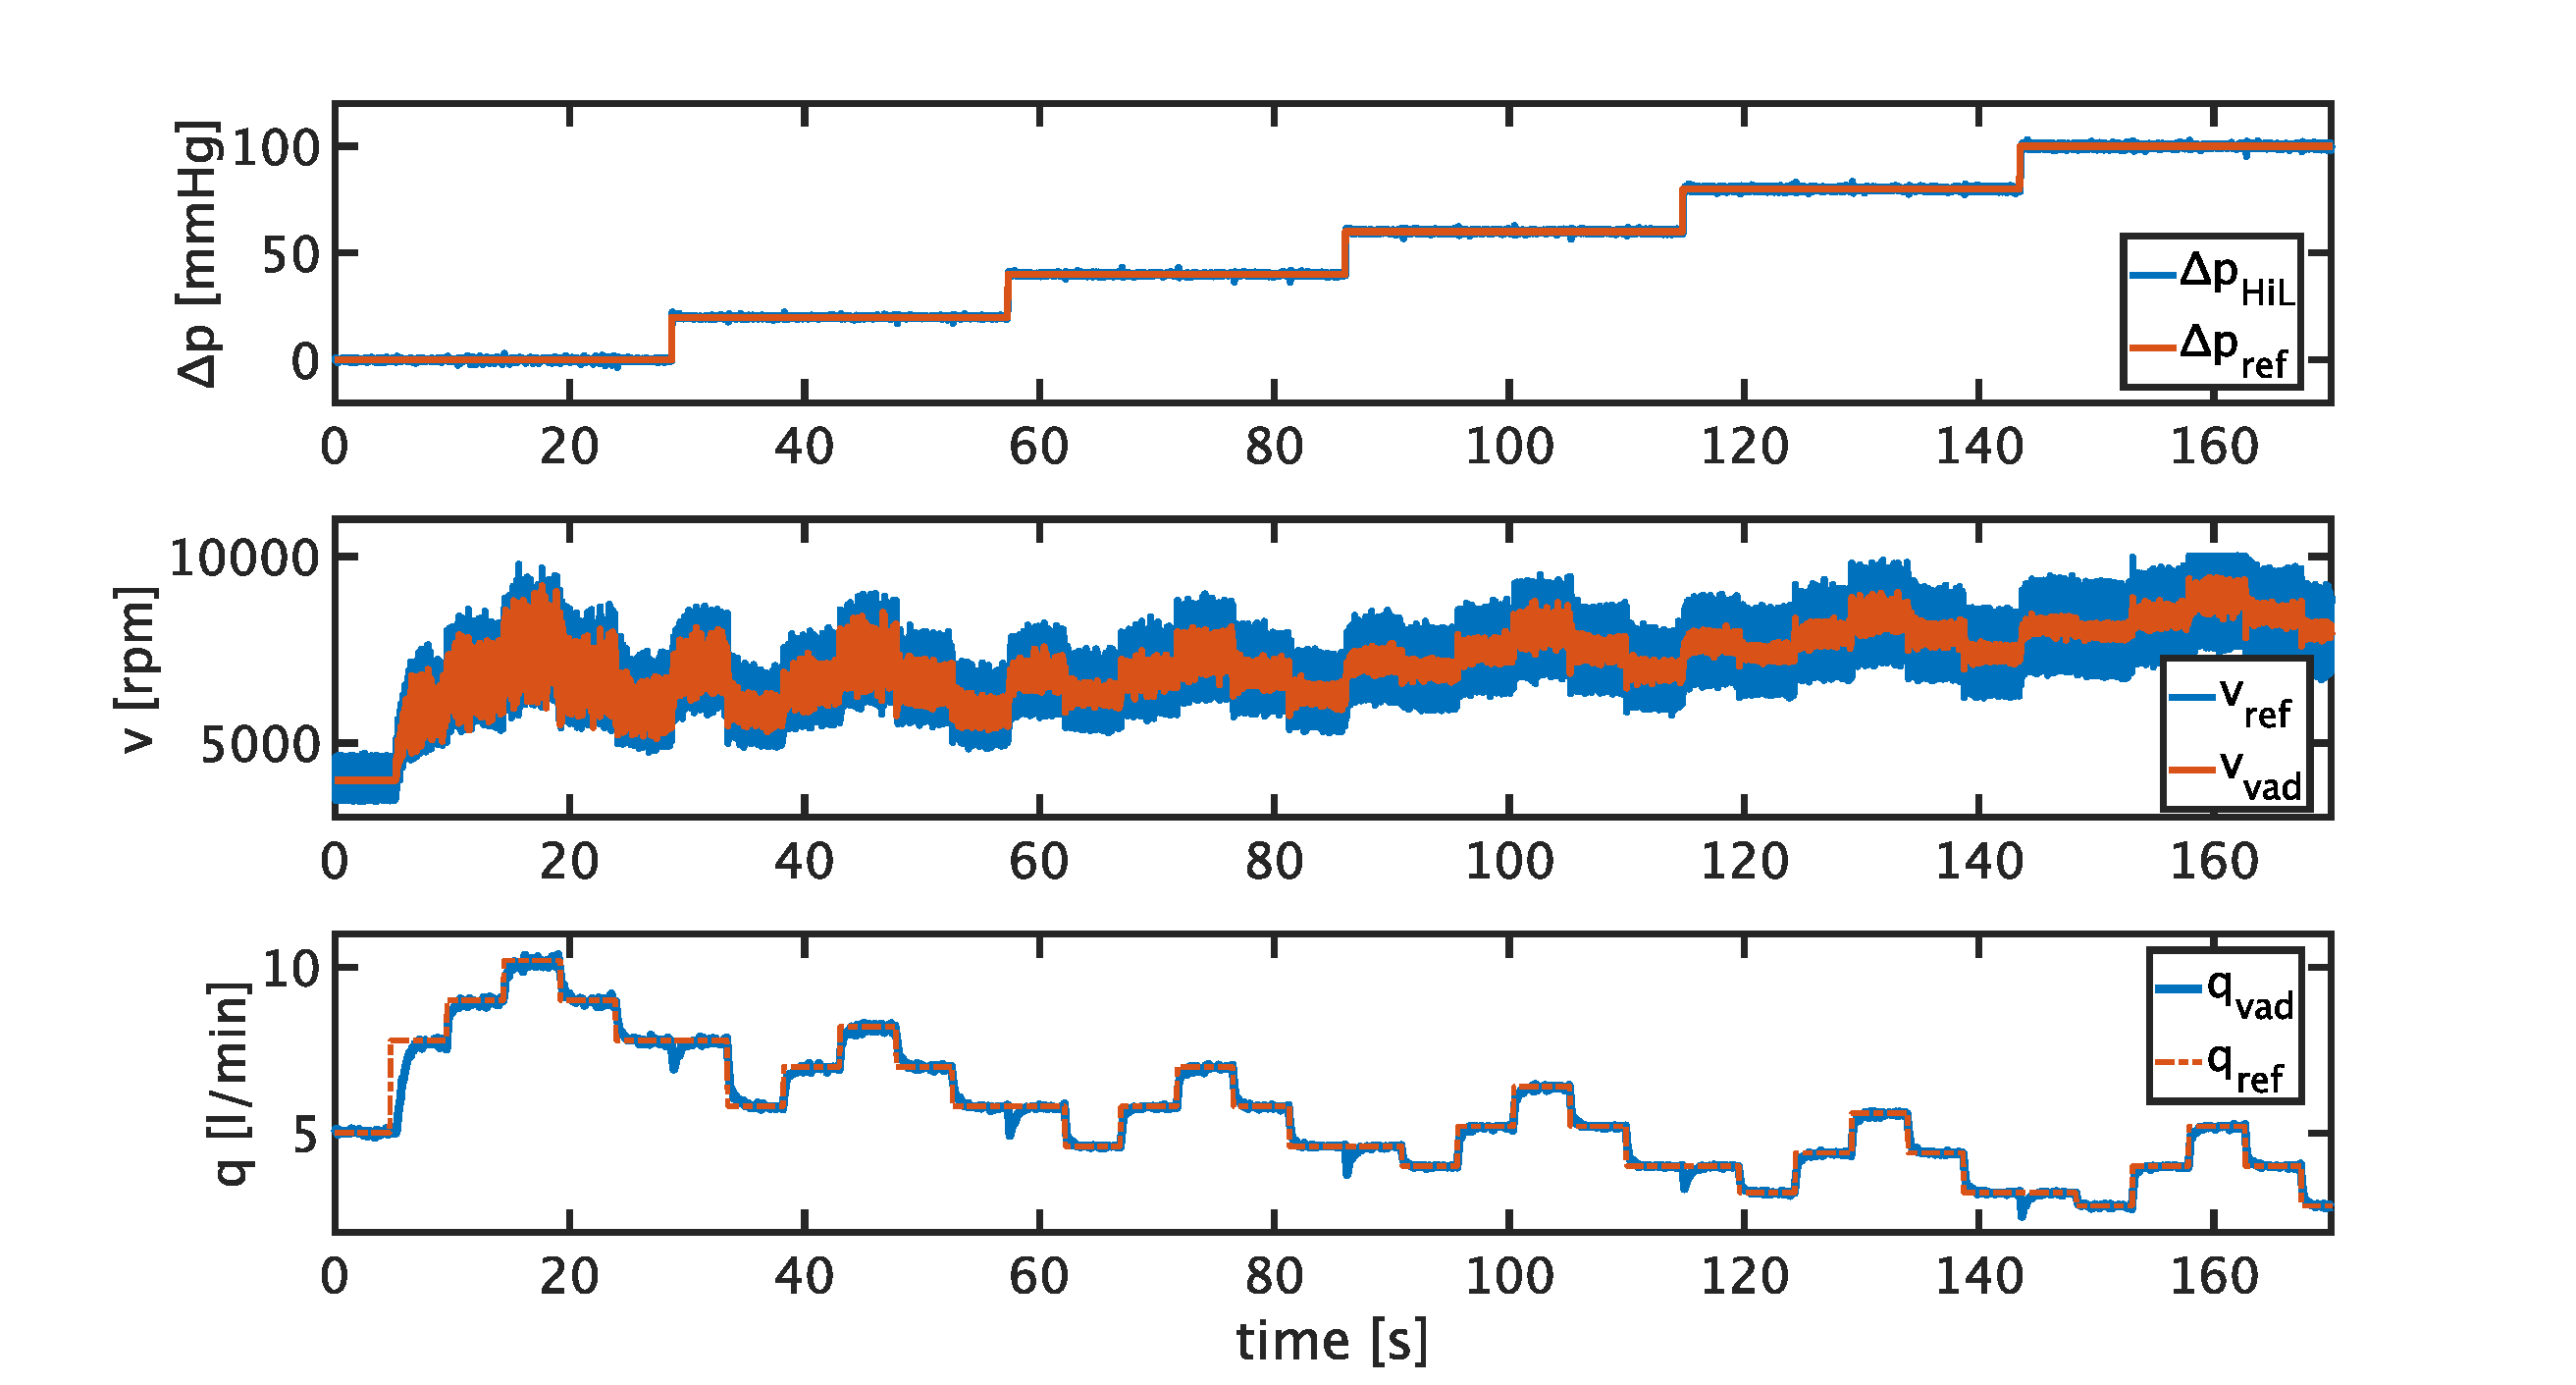
\includegraphics[width=\textwidth]{images/chapt_5/pi_contr_chr.pdf}
  \caption[Step response for determination of PI controller tuning parameters]{Step response for a step in rotational speed of $400\,rpm$ for determination of PI controller tuning parameters.}
  \label{fig:pi_contr_chr}
\end{figure}

% \begin{figure}[ht]
%   \centering
%   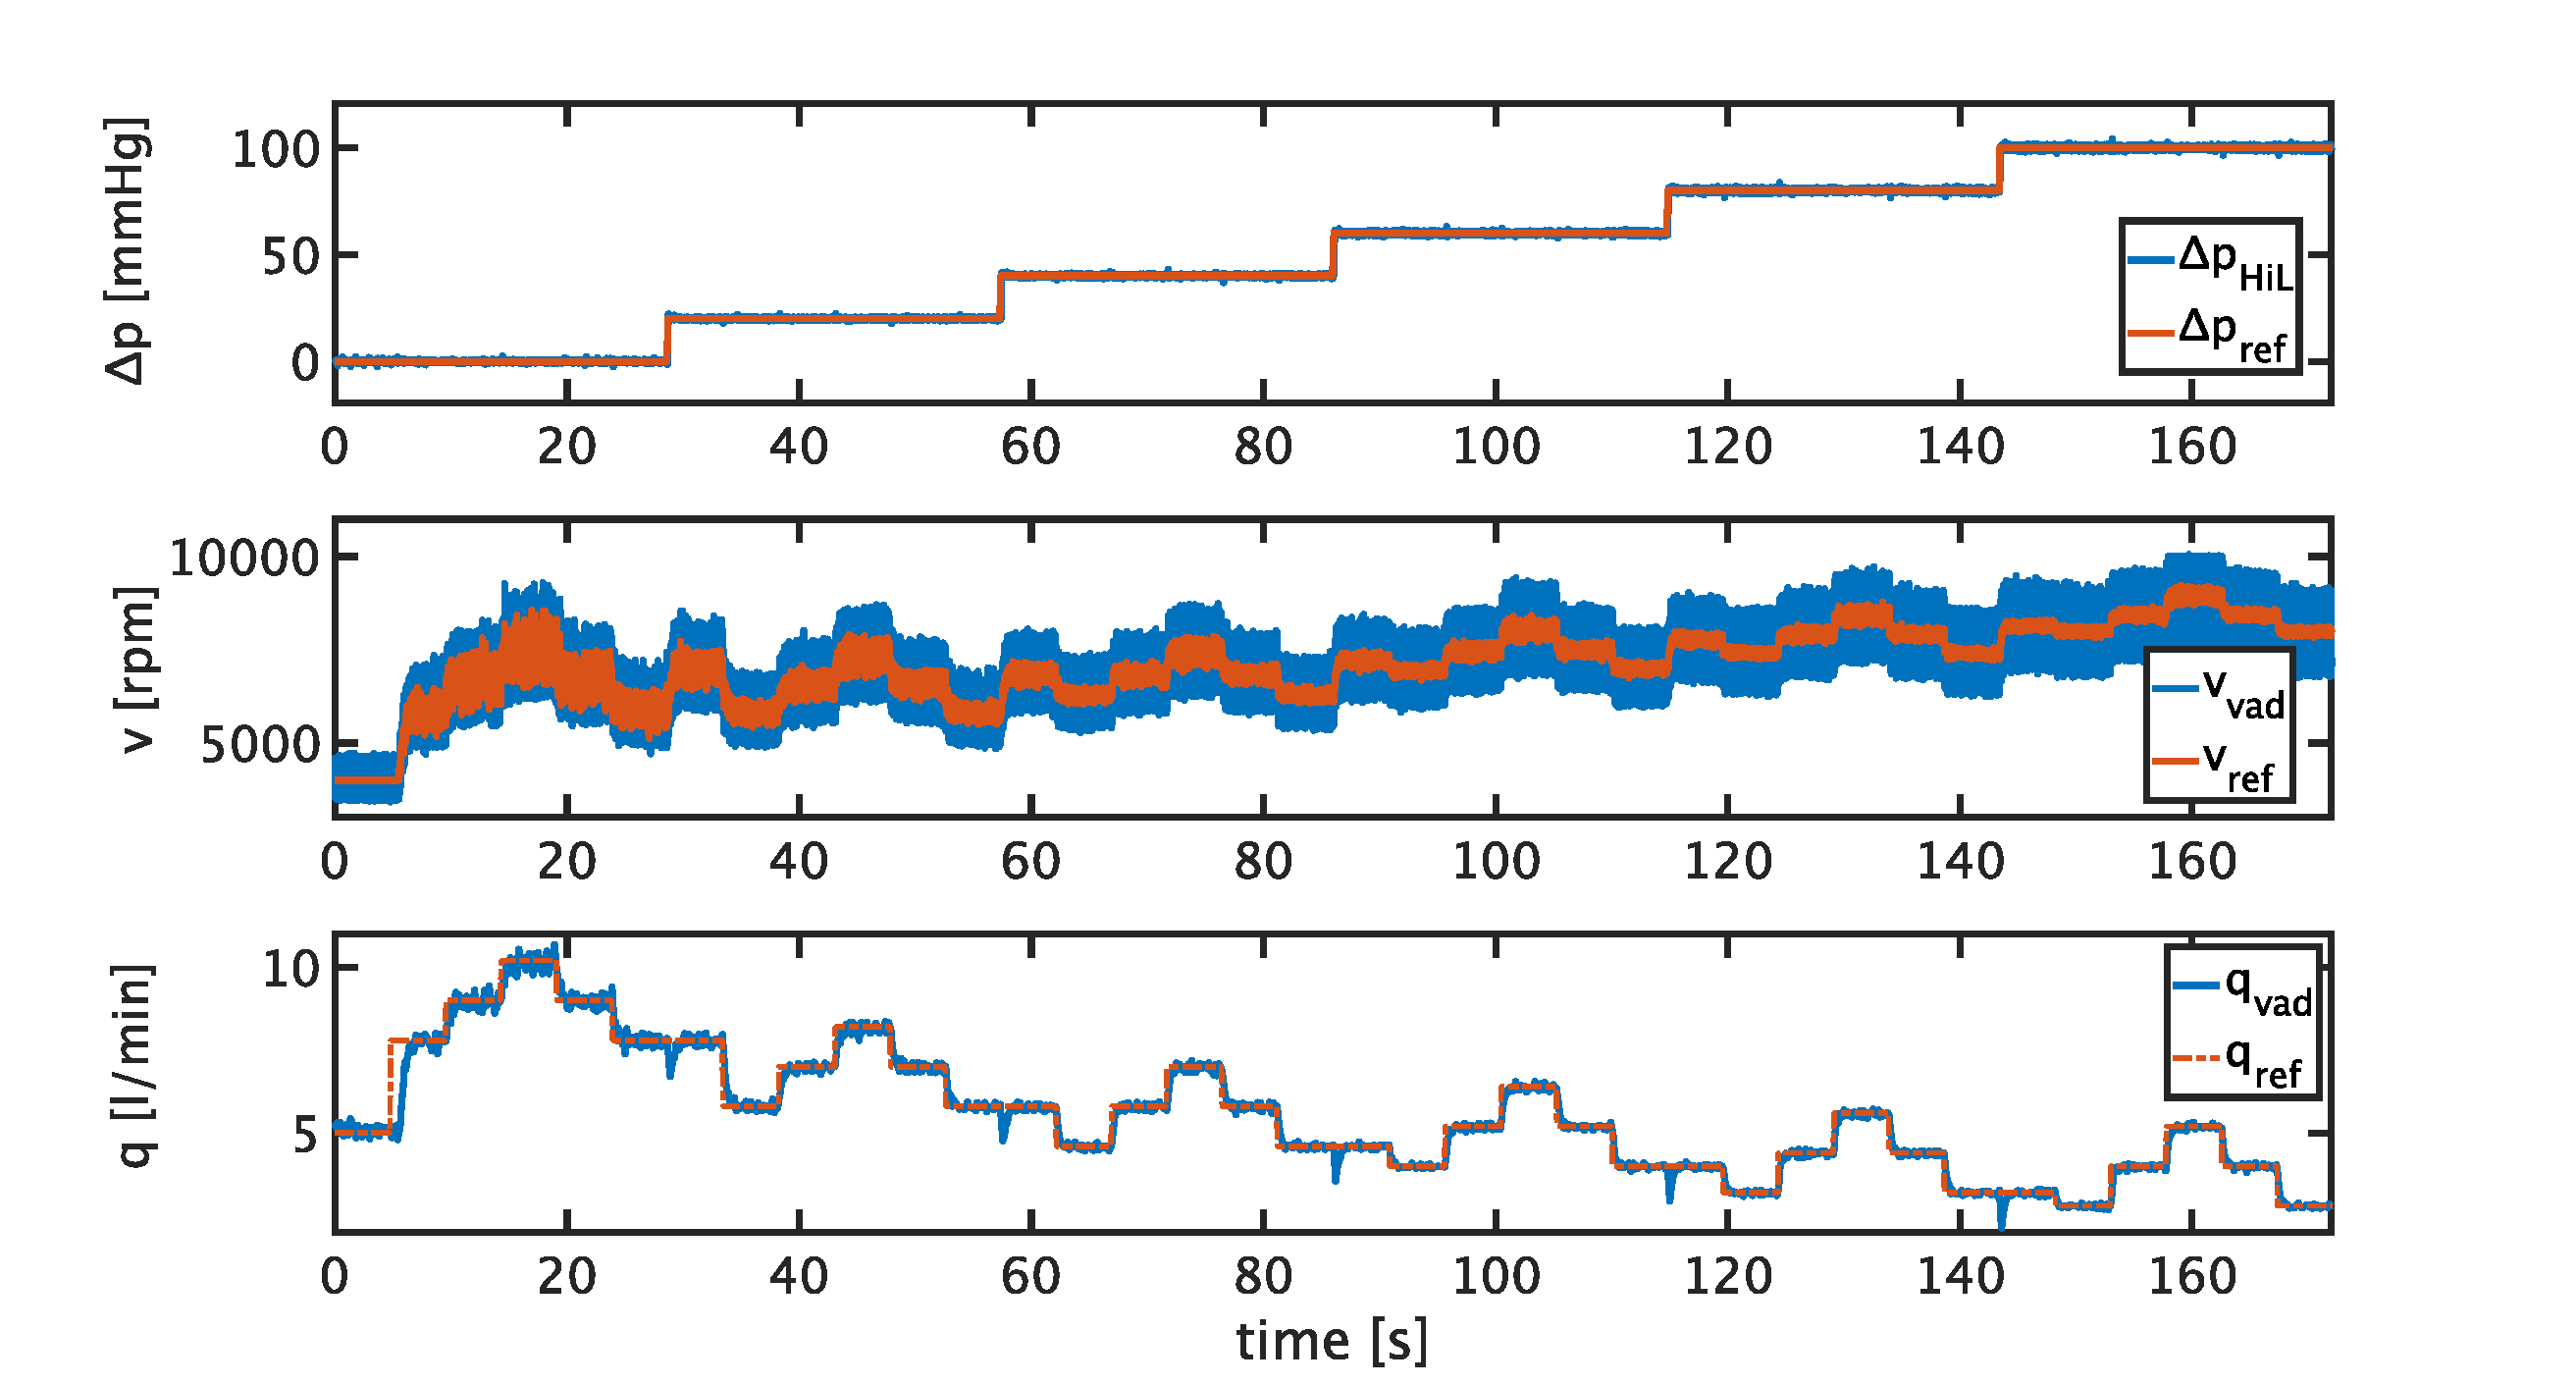
\includegraphics[width=\textwidth]{images/chapt_5/pi_contr_zn.pdf}
%   \caption[Step response for determination of PI controller tuning parameters]{Step response for a step in rotational speed of $400\,rpm$ for determination of PI controller tuning parameters.}
%   \label{fig:pi_contr_zn}
% \end{figure}

Bereich der Auslegung: 40mmHg
RMS PI CHR = 0.2753
RMS PI ZN = 0.4013

% \begin{figure}[ht]
%   \centering
%   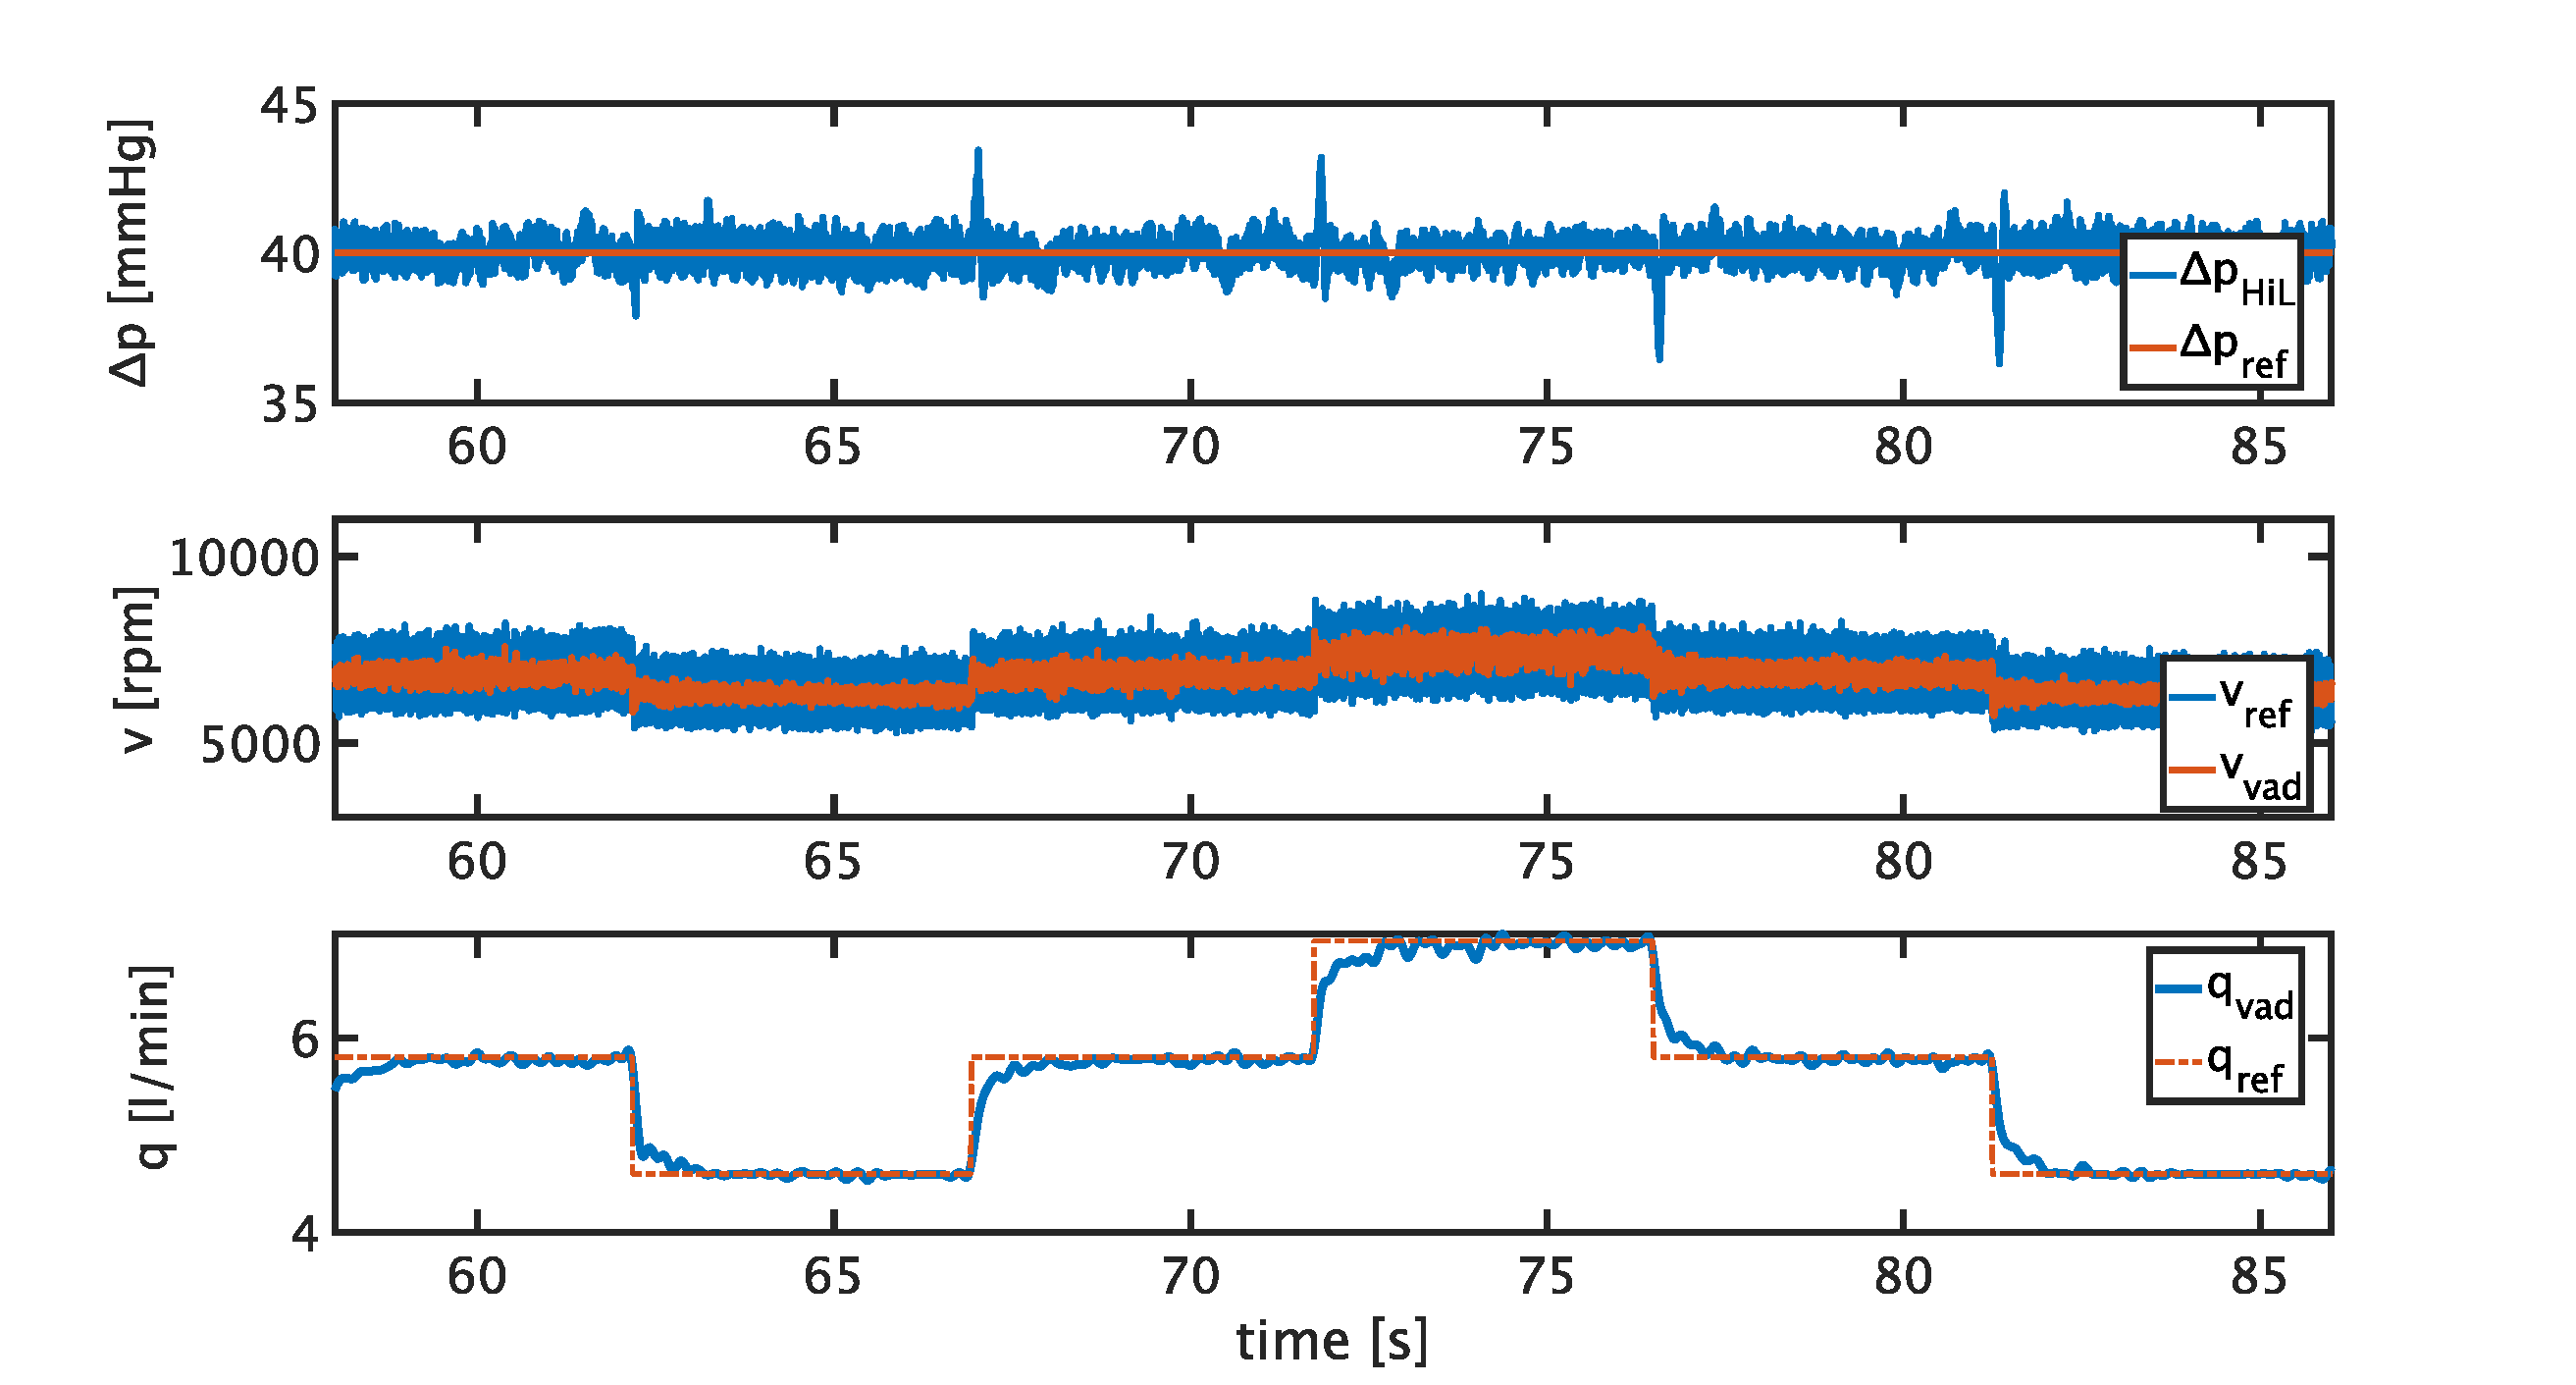
\includegraphics[width=\textwidth]{images/chapt_5/pi_contr_chr_40.pdf}
%   \caption[Step response for determination of PI controller tuning parameters]{Step response for a step in rotational speed of $400\,rpm$ for determination of PI controller tuning parameters.}
%   \label{fig:pi_contr_chr_40}
% \end{figure}

\begin{figure}[ht]
  \centering
  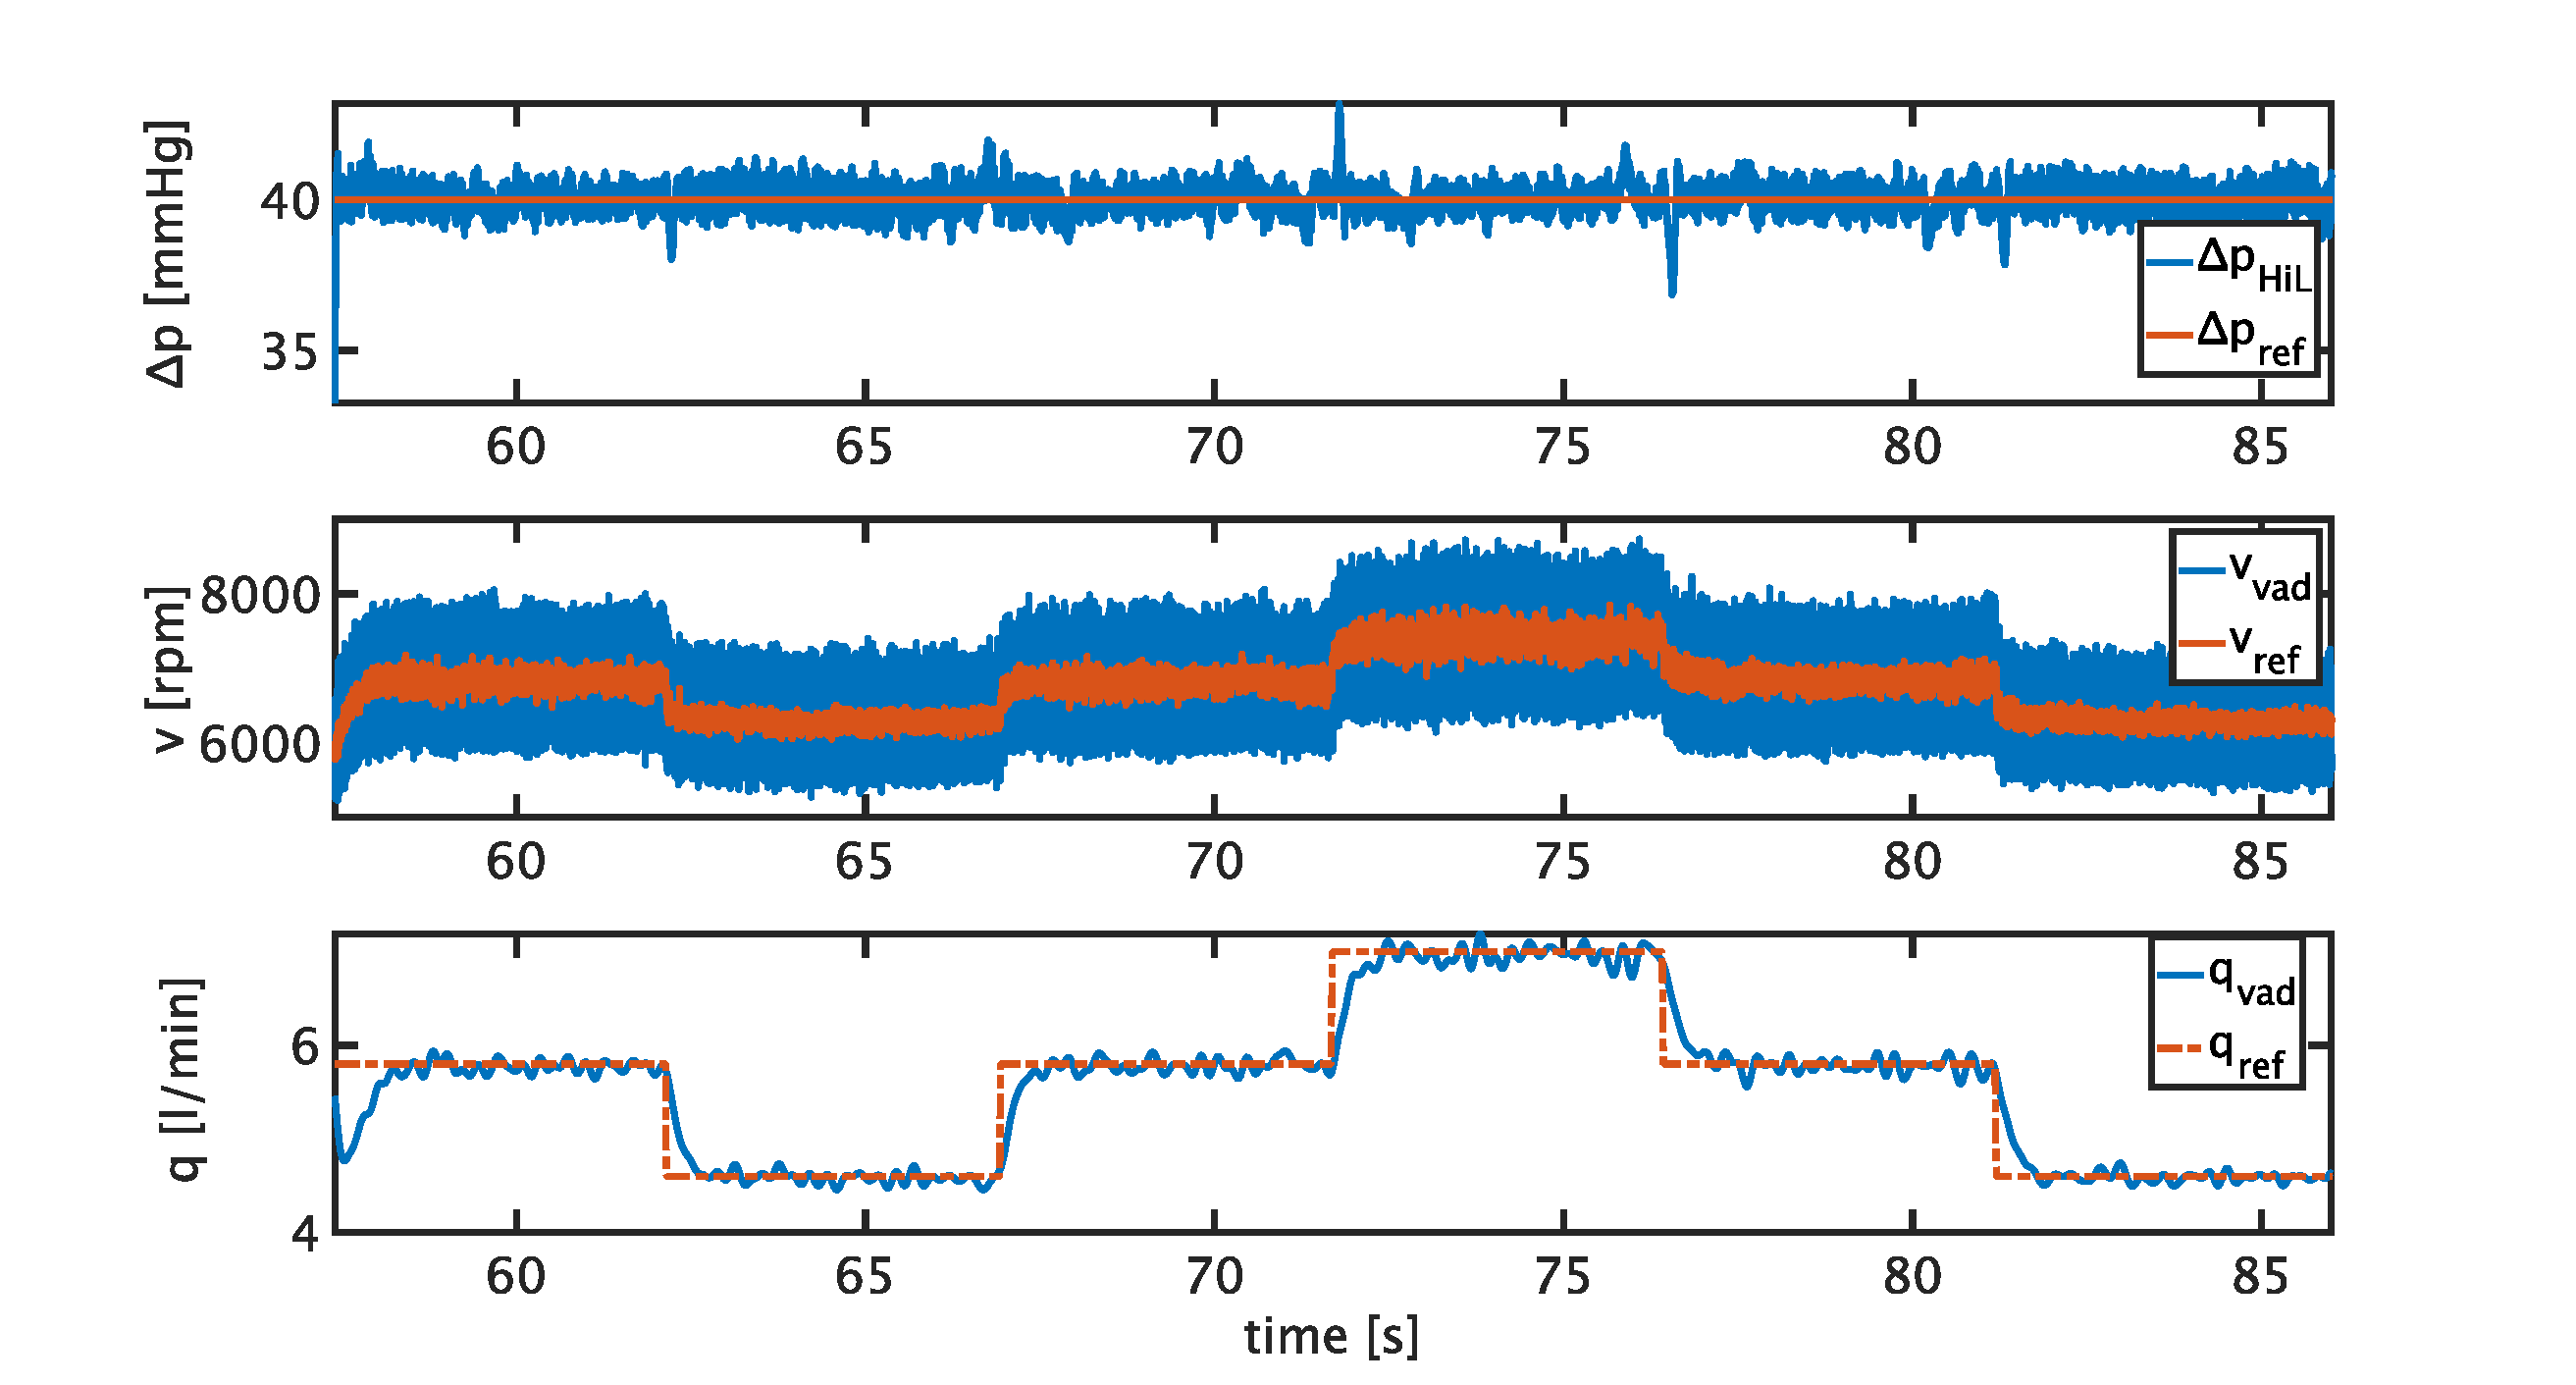
\includegraphics[width=\textwidth]{images/chapt_5/pi_contr_zn_40.pdf}
  \caption[Step response for determination of PI controller tuning parameters]{Step response for a step in rotational speed of $400\,rpm$ for determination of PI controller tuning parameters.}
  \label{fig:pi_contr_zn_40}
\end{figure}
\subsubsection{Chien Hrones Reswick}
% Dynamische Messung nutzen
% Werte an Sprungstellen
% Nach Wendetangenten verfahren -> GRAFIK
%Berechnung erklären
\subsection{Iterative Learning Control}
\subsection{Iterative Learning Control with varying iteration length}
% Kontanten Fluss über verschiedene Druckbereiche?
%
% %Druckverlauf ohne Störung
%
% Herzschlag dazu - Druckverlauf
